\documentclass{article}
\usepackage{xeCJK, amsmath, amssymb, geometry, graphicx, float}
\setCJKmainfont{標楷體}
\geometry{a4paper, margin=2.5cm}

\title{數統導論作業五}
\author{111020003 林群佑}
\date{}

\begin{document}
\maketitle
\section*{4.1.2}

\subsection*{(a)}

The histogram of the 26 professional baseball pitchers' weights is shown in Figure \ref{fig:histogram}.

\begin{figure}[H]
    \centering
    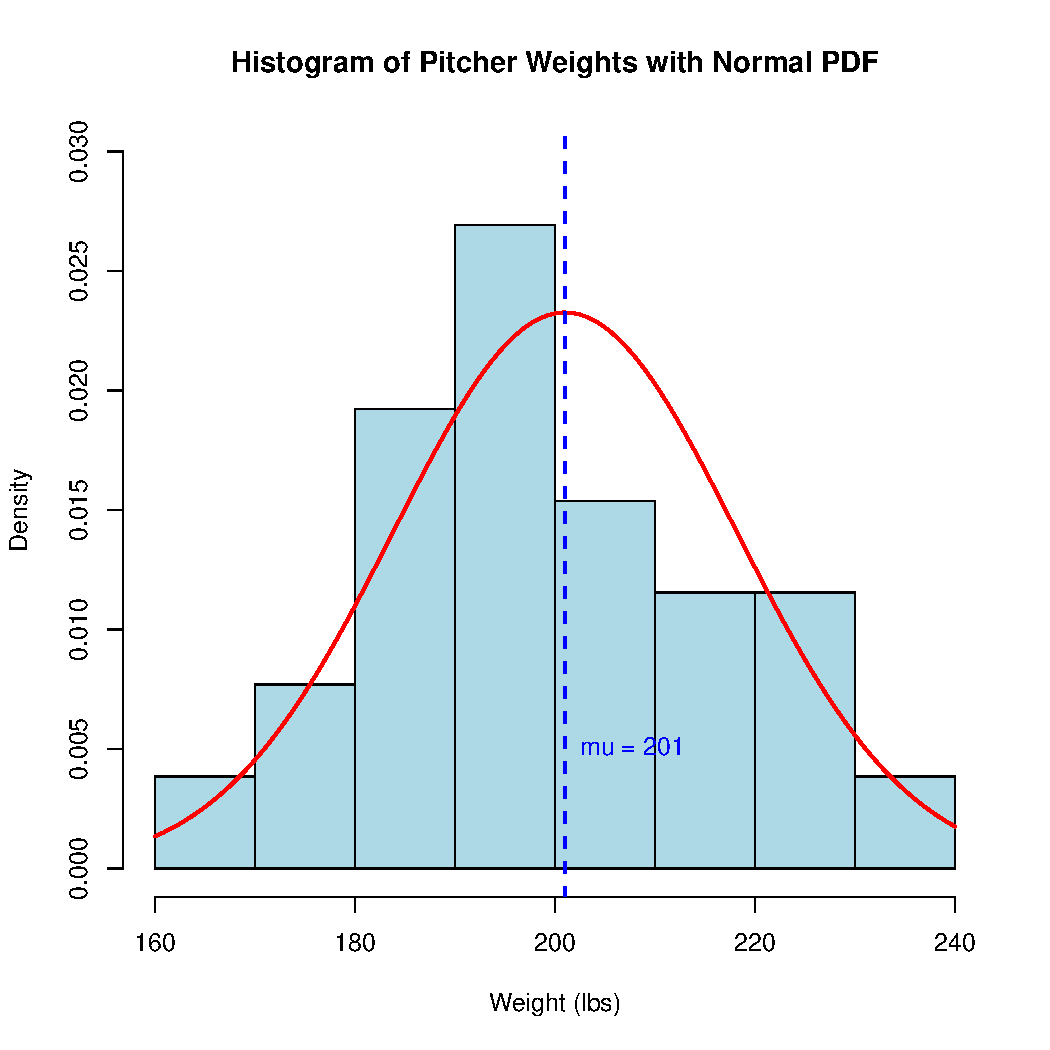
\includegraphics[width=0.7\textwidth]{pitcher_hist.pdf} 
    \caption{Histogram of pitcher weights with overlaid normal PDF.}
    \label{fig:histogram}
\end{figure}

\noindent
Based on the plot, the data appears roughly symmetric and bell-shaped. Although the sample size ($n=26$) is small, the normal probability model seems credible.

\subsection*{(b)}

Let $X_1, X_2, \dots, X_n$ be a random sample from a normal distribution 
$N(\mu, \sigma^2)$. The probability density function is:
\[
f(x; \mu, \sigma^2) = \frac{1}{\sqrt{2\pi\sigma^2}} \exp\left\{-\frac{(x-\mu)^2}{2\sigma^2}\right\}
\]

The likelihood function is given by:
\begin{align*}
L(\mu, \sigma^2) &= \prod_{i=1}^n f(x_i; \mu, \sigma^2) \\
&= \prod_{i=1}^n \left( (2\pi\sigma^2)^{-1/2} \exp\left\{-\frac{(x_i-\mu)^2}{2\sigma^2}\right\} \right) \\
&= (2\pi\sigma^2)^{-n/2} \exp\left\{-\frac{1}{2\sigma^2}\sum_{i=1}^n (x_i-\mu)^2\right\}
\end{align*}

The log-likelihood function is:
\[
l(\mu, \sigma^2) = \ln L(\mu, \sigma^2) = -\frac{n}{2}\ln(2\pi) - \frac{n}{2}\ln(\sigma^2) - \frac{1}{2\sigma^2}\sum_{i=1}^n (x_i-\mu)^2
\]

To find the MLEs, we differentiate $l(\mu, \sigma^2)$ with respect to $\mu$ and $\sigma^2$, and set the derivatives to zero.

\textbf{1. For $\mu$:}
\begin{align*}
\frac{\partial l}{\partial \mu} &= \frac{1}{\sigma^2}\sum_{i=1}^n (x_i-\mu) = 0 \\
\sum_{i=1}^n x_i - n\mu &= 0 \quad \Rightarrow \quad \hat{\mu} = \frac{1}{n}\sum_{i=1}^n x_i = \bar{X}
\end{align*}

\textbf{2. For $\sigma^2$:}
\begin{align*}
\frac{\partial l}{\partial \sigma^2} &= -\frac{n}{2\sigma^2} + \frac{1}{2(\sigma^2)^2}\sum_{i=1}^n (x_i-\mu)^2 = 0 \\
\frac{n}{2\sigma^2} &= \frac{1}{2(\sigma^2)^2}\sum_{i=1}^n (x_i-\mu)^2 \\
n &= \frac{1}{\sigma^2}\sum_{i=1}^n (x_i-\hat{\mu})^2 \quad \Rightarrow \quad \hat{\sigma}^2 = \frac{1}{n}\sum_{i=1}^n (x_i-\bar{X})^2
\end{align*}

Based on the data ($n=26$):
\begin{itemize}
    \item $\hat{\mu} = \frac{5226}{26} =201$
    \item $\hat{\sigma}^2 = \frac{7642}{26} \approx 293.923$
    \item By the invariance property of MLE: $\hat{\sigma} \approx \sqrt{293.923} \approx 17.144$
    \item $\widehat{\mu/\sigma} \approx 201 / 17.144 \approx 11.724$
\end{itemize}
The estimate of $\mu$ is located at the center of the symmetry in Figure \ref{fig:histogram}.

\subsection*{(c)}

Let $Y$ be the random variable representing the number of pitchers weighing 
over 215 pounds. We model $Y$ using a binomial distribution 
$Y \sim \text{Bin}(n, p)$, where $n=26$ and $p$ is the unknown probability 
of success.

\noindent
The probability mass function (PMF) is given by:
\[
P(Y=y) = \binom{n}{y} p^y (1-p)^{n-y}
\]
The likelihood function for the parameter $p$ given the observation $y$ is:
\[
L(p) = \binom{n}{y} p^y (1-p)^{n-y}
\]
The log-likelihood function is:
\begin{align*}
l(p) = \ln L(p) &= \ln \left[ \binom{n}{y} p^y (1-p)^{n-y} \right] \\
&= \ln \binom{n}{y} + y \ln p + (n-y) \ln(1-p)
\end{align*}
To find the maximum likelihood estimate $\hat{p}$, we differentiate $l(p)$ with respect to $p$ and set the derivative to zero:
\begin{align*}
\frac{d l(p)}{d p} &= 0 + \frac{y}{p} - \frac{n-y}{1-p} = 0 \\
\frac{y}{p} &= \frac{n-y}{1-p} \\
y(1-p) &= p(n-y) \\
y - yp &= np - yp \\
y &= np \\
\hat{p} &= \frac{y}{n}
\end{align*}

\noindent
Based on the data, the weights over 215 lbs are: 218, 219, 220, 222, 225, 225, 232.
\begin{itemize}
    \item Number of successes ($y$): 7
    \item Total sample size ($n$): 26
\end{itemize}

Substituting these values into the MLE estimator:
\[
\hat{p} = \frac{7}{26} \approx 0.2692
\]

\noindent
Thus, the estimated proportion of professional baseball pitchers who weigh over 215 pounds is 
approximately 26.9\%.

\section*{4.1.3}
\subsection*{(a)}
Let $X_1, X_2, \dots, X_n$ be a random sample from a Poisson distribution 
$\text{Poisson}(\theta)$. The probability mass function is:
\[
f(x; \theta ) = \frac{e^{-\theta} \theta^x }{x!}
\]
The likelihood function is given by:
\begin{align*}
L(\theta) &= \prod_{i=1}^n f(x_i; \theta )\\
&= \prod_{i=1}^n \frac{e^{-\theta} \theta^{x_i} }{x_i!}\\
&= \frac{e^{-n\theta} \theta^{\sum_{i=1}^{n} x_i}}{\prod_{i=1}^n x_i!}
\end{align*}
The log-likelihood function is:
\begin{align*}
l(\theta) = \ln L(\theta) &= 
\ln \left[\frac{e^{-n\theta} \theta^{\sum_{i=1}^{n} x_i}}{\prod_{i=1}^n x_i!}\right]\\
&= -n \theta + \left(\sum_{i=1}^{n} x_i\right) \ln \theta - \ln \left(\prod_{i=1}^n x_i!\right)
\end{align*}
To find the maximum likelihood estimate $\hat{\theta}$, we differentiate $l(\theta)$ with respect 
to $\theta$ and set the derivative to zero:
\begin{align*}
\frac{d l(\theta)}{d \theta} &= -n + \frac{\sum_{i=1}^{n} x_i}{\theta} - 0 = 0\\
n &= \frac{\sum_{i=1}^{n} x_i}{\theta}\\
n \theta &= \sum_{i=1}^{n} x_i\\
\hat{\theta} &= \frac{1}{n} \sum_{i=1}^{n} x_i = \bar{X}
\end{align*}
Next, we show that $\hat{\theta}_{MLE}$ is an unbiased estimator:
\[
E[\hat{\theta}_{MLE}] = E\left[\frac{1}{n} \sum_{i=1}^{n} X_i\right] = 
\frac{1}{n}\sum_{i=1}^{n} E\left[ X_i\right]
\]
Since $X_i \sim \text{Poisson}(\theta)$, we know that $E[X_i] = \theta$.
\[
E[\hat{\theta}_{MLE}] = \frac{1}{n}\sum_{i=1}^{n} \theta = \frac{n \theta}{n}= \theta
\]
We have proved that $E[\hat{\theta}_{MLE}] = \theta$. Therefore, the MLE of the Poisson 
distribution is an unbiased estimator.

\subsection*{(b)}
Given the data, we calculate the estimate:
\[
\hat{\theta}_{MLE} = \frac{1}{10} (9+7+9+15+10+13+11+7+2+12) = \frac{95}{10} = 9.5
\]
This means that, on average, 9.5 customers enter the store between 9:00 a.m. and 10:00 a.m.
\section*{5.1.1}
\subsection*{(1) Show that $a_n \to a \implies a_n \xrightarrow{P} a$}
Assume $a_n \to a$.
\begin{enumerate}
    \item By  definition of $a_n \to a$ we have $\forall \, \epsilon > 0 , 
    \, \exists N \text{ that }\forall n > N \text{ we have }\left|a_n - a\right|<\epsilon$
    \item Therefore, $\forall n > N$:
    \[
    P\left(\left|a_n - a\right| \ge \epsilon\right) = P(\emptyset) = 0
    \]
    \item Taking the limit as $n \to \infty$:
    \[
    \lim_{n \rightarrow \infty} P\left(|a_n - a| \ge \epsilon\right) = 0
    \]
    \item Thus, $a_n \xrightarrow{P} a$.
\end{enumerate}
\subsection*{(2) Show that $a_n \xrightarrow{P} a \implies a_n \to a$}
Assume $a_n \xrightarrow{P} a$.
\begin{enumerate}
    \item By definition we have:
    \[
    \forall \epsilon > 0 , \, 
    \lim_{n \rightarrow \infty} P\left(\left|a_n - a\right| \ge \epsilon\right) = 0
    \]
    \item Note that since $a_n$ is a constant sequence, the variable $|a_n - a|$ is deterministic. Thus, the probability $P(|a_n - a| \ge \epsilon)$ can only take values in $\{0, 1\}$.
    \[
    P(|a_n - a| \ge \epsilon) = \begin{cases} 
    1 & \text{if } |a_n - a| \ge \epsilon \\
    0 & \text{if } |a_n - a| < \epsilon 
    \end{cases}
    \]
    \item A sequence taking values in $\{0, 1\}$ that converges to 0 must clearly be equal to 0 for all sufficiently large $n$.
    \item Therefore, $\exists N \in \mathbb{N}$ such that $\forall n \ge N$:
    \[
    P\left(|a_n - a| \ge \epsilon\right) = 0
    \]
    \item This implies that for all $n \ge N$, the condition $|a_n - a| \ge \epsilon$ is false, which means:
    \[
    |a_n - a| < \epsilon
    \]
    \item This satisfies the definition of $a_n \to a$.
\end{enumerate}
\subsection*{(3) Conclusion}
We proved that:
\[
    a_n \xrightarrow{P} a \iff a_n \to a ,\text{ when } a \in \mathbb{R}
\]
\section*{5.1.2}
\subsection*{(a)}
Since $Y_n \sim b(n, p)$, we have :
\[
    \mathbb{E}[Y_n] = np ,\, Var(Y_n) = np(1-p) \implies
    \mathbb{E}\left[\frac{Y_n}{n}\right] = p ,\, Var\left(\frac{Y_n}{n}\right) = \frac{p(1-p)}{n}
\]
By Chebyshev's inequality $\forall \, \epsilon > 0$ :
\[
P\left(\left|\frac{Y_n}{n} - \mathbb{E}\left[\frac{Y_n}{n}\right]\right| \ge \epsilon \right) \le 
\frac{Var\left(\frac{Y_n}{n}\right)}{\epsilon^2} \implies
P\left(\left|\frac{Y_n}{n} - p\right| \ge \epsilon \right) \le \frac{p(1-p)}{n \epsilon^2}
\]
Take limit as $n \rightarrow \infty$ :
\[
\lim_{n \rightarrow \infty}P\left(\left|\frac{Y_n}{n} - p\right| \ge \epsilon \right) \le 
\lim_{n \rightarrow \infty} \frac{p(1-p)}{n \epsilon^2} = 0
\]
Also, we know that probability is a value in closed interval $[0,1]$.\\
By squeeze theorem :
\[
0 \le \lim_{n \rightarrow \infty}P\left(\left|\frac{Y_n}{n} - p\right| \ge \epsilon \right) \le 
\lim_{n \rightarrow \infty} \frac{p(1-p)}{n \epsilon^2} = 0 \implies 
\lim_{n \rightarrow \infty}P\left(\left|\frac{Y_n}{n} - p\right| \ge \epsilon \right) = 0,
\quad \forall \, \epsilon > 0
\]
Thus, $Y_n / n$ converges in probability to p.
\subsection*{(b)}
$\forall \, \epsilon > 0$, we have :
\[
\lim_{n \rightarrow \infty}P\left(\left|\left(1-\frac{Y_n}{n}\right) 
- (1-p)\right| \ge \epsilon \right) = 
\lim_{n \rightarrow \infty}P\left(\left|p-\frac{Y_n}{n}\right| \ge \epsilon \right)
= \lim_{n \rightarrow \infty}P\left(\left|\frac{Y_n}{n}-p\right| \ge \epsilon \right)
\]
By previous problem we have :
\[
\lim_{n \rightarrow \infty}P\left(\left|\frac{Y_n}{n}-p\right| \ge \epsilon \right) = 0 ,
\quad \forall \, \epsilon > 0 
\]
Therefore, $\forall \, \epsilon > 0$ :
\[
\lim_{n \rightarrow \infty}P\left(\left|\left(1-\frac{Y_n}{n}\right) 
- (1-p)\right| \ge \epsilon \right) = 0
\]
Which means that $1-Y_n / n$ converges in probability to $1-p$.
\subsection*{(c)}
By Slutsky's Theorem :
\[
\frac{Y_n}{n} \xrightarrow{P} p \text{ and }
1-\frac{Y_n}{n} \xrightarrow{P} 1-p \implies 
\left(\frac{Y_n}{n}\right)\left(1-\frac{Y_n}{n}\right) \xrightarrow{P}
p(1-p)
\]
\section*{5.1.3}
By Chebyshev's inequality, $\forall \, \epsilon > 0$ :
\[
P\left(\left|W_n - E\left[ W_n \right]\right|\ge\epsilon\right) \le
\frac{Var\left(W_n\right)}{\epsilon^2} \implies
P\left(\left|W_n - \mu\right|\ge\epsilon\right)\le\frac{b}{n^p \epsilon^2}
\]
Take limit as $n \to \infty$ :
\[
    \lim_{n \rightarrow \infty}P\left(\left|W_n - \mu\right|\ge\epsilon\right)\le
    \lim_{n \rightarrow \infty}\frac{b}{n^p \epsilon^2} = 0
\]
Also, we know that probability is a value in closed interval $[0,1]$.\\
By squeeze theorem :
\[
0 \le
\lim_{n \rightarrow \infty}P\left(\left|W_n - \mu\right|\ge\epsilon\right)\le
\lim_{n \rightarrow \infty}\frac{b}{n^p \epsilon^2} = 0 \implies
\lim_{n \rightarrow \infty}P\left(\left|W_n - \mu\right|\ge\epsilon\right) = 0,
\quad \forall \, \epsilon > 0
\]
Thus, $W_n$ converges in probability to $\mu$.
\section*{5.1.4}
Let $Y_n = \max\{X_1, \dots, X_n\}$. By the definition of the CDF:
\begin{align*}
F_{Y_n}(t) &= P(Y_n < t)\\
&= P\left(max(X_1,X_2 \dots X_n) < t\right)\\
&= P\left(X_1 < t, X_2 < t \dots X_n < t\right)
\end{align*}
Since $X_1, \dots, X_n$ are independent and identically distributed with CDF $F_X(t)$, 
we have:
\begin{align*}
F_{Y_n}(t) &= \prod_{i=1}^{n} P\left(X_i < t\right) =  [F_X(t)]^n
\end{align*}
Substituting the CDF of the Uniform$(0, \theta)$ distribution :
$$
F_X(t) = 
\begin{cases}
    1 & t > \theta \\
    \frac{t}{\theta} & 0 < t \le \theta \\
    0 & t \le 0
\end{cases}
$$
We obtain:
\[
F_{Y_n}(t) = 
\begin{cases}
    1^n = 1 & t > \theta\\
    \left(\frac{t}{\theta}\right)^n  & 0 < t \le \theta \\
    0^n = 0 & t \le 0
\end{cases}
\]
Therefore, we provd that :
\[
F_{Y_n}(t) = 
\begin{cases}
    1 & t > \theta\\
    \left(\frac{t}{\theta}\right)^n  & 0 < t \le \theta \\
    0 & t \le 0
\end{cases}
\]
\section*{5.2.1}
Since $X_1, ..., X_n$ is a random sample from $N(\mu, \sigma^2)$, 
the sample mean has the distribution $\bar{X}_n \sim N(\mu, \sigma^2/n)$.
The moment generating function (MGF) of $\bar{X}_n$ is:
$$
M_{\bar{X}_n}(t) = \exp\left(\mu t + \frac{\sigma^2 t^2}{2n}\right)
$$
Taking the limit as $n \to \infty$:
$$
\lim_{n \to \infty} M_{\bar{X}_n}(t) = e^{\mu t}
$$
Since $e^{\mu t}$ is the MGF of a degenerate distribution with all probability mass at $\mu$, 
the limiting distribution of $\bar{X}_n$ is a degenerate distribution at $\mu$.
\end{document}